\chapter[Revisão Bibliográfica]{Revisão Bibliográfica}
\label{fundamentacao}
% ----------------------------------------------------------
%Ataques distribuídos de negação de serviço (do inglês, DDoS) figuram uma das principais ameaças de segurança atualmente. Organizações perdem financeiramente e principalmente tendem a ter seu valor questionado quando são vítimas de invasores na rede.
Nesse capítulo, os conceitos acerca deste trabalho são apresentados, abordando definições na área de segurança em redes tais como ataques DoS, DDoS, sistemas IDS, além de uma revisão da literatura acerca de \textit{frameworks} de detecção de ataques em redes de computadores. 
\section{Segurança da Informação}
Uma ameaça trata-se de um potencial para violação de segurança quando há uma circunstância que pode quebrá-la, causando danos a um serviço/\textit{host}. Exemplos de ameaças são: \textit{malwares}, ataques de negação de serviço e envio de pacotes com falso endereço origem. Uma ameaça explora uma vulnerabilidade no alvo para obter as informações que deseja ou mesmo tornar o serviço indisponível, ou seja, ocorrendo a violação da segurança no alvo que é o ataque. Um ataque pode ocasionar, por exemplo, a destruição dos dados, perda da integridade, dentre outros incidentes. Um incidente, por sua vez pode causar prejuízo financeiro para a imagem do alvo, além de causar indisponibilidade do serviço fornecido \cite{kurose}. A \figref{fig:ameacas} mostra uma síntese desses conceitos.   

 \begin{figure}[ht]
 	\centering
 	\caption{Fluxo explicativo de uma ameaça }
 	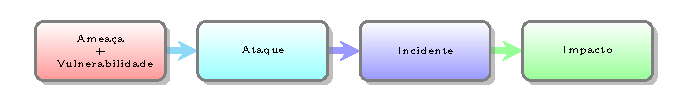
\includegraphics[width=1\textwidth]{figs/ameacas.pdf}\\
 	{Fonte: Elaborada pelo autor.}
 	\label{fig:ameacas}
 \end{figure}
 
 \section{Ataques DoS e DDoS}

Um ataque de negação de serviço (DoS - Denial-of-Service) torna um componente de rede inutilizável por usuários que estejam consumindo o serviço fornecido. A maioria dos ataques DoS na \textit{internet} pode ser dividida em três categorias: \cite{kurose}
\begin{itemize}
	\item Ataque de vulnerabilidade: Mensagens são enviadas a uma aplicação vulnerável ou a um servidor, sendo executado em um hospedeiro alvo.
	\item Inundação na largura de banda: O atacante envia um grande número de pacotes maliciosos ao hospedeiro alvo até que o enlace de acesso do alvo fique cheio, impedindo os pacotes legítimos de alcançarem o servidor. 
	\item Inundação na conexão: O atacante estabelece um grande número de conexões TCP semiabertas ou abertas no hospedeiro alvo. 
\end{itemize}

Já segundo \citeonline{ddosatacks}, os ataques DoS são classificados em cinco categorias baseadas no protocolo cujo é atacado: dispositivo, sistema operacional, aplicação, inundação de dados e características do protocolo. O primeiro inclui ataques que podem ser causados ao tirar vantagem de \textit{bugs} ou vulnerabilidades em \textit{software}. O segundo leva em consideração, ataques que aproveitam-se da forma como os protocolos são implementados pelos sistemas operacionais. Ataques baseados na aplicação infectam o alvo por meio de \textit{bugs} específicos da rede e tentam drenar os recursos da vítima. Em ataques baseados em inundação de dados, um atacante tenta usar a largura de banda disponível para mandar grandes quantidades de dados, fazendo com que o alvo processe todo esse volume de informação. Por fim, ataques baseados em características do protocolo são caracterizados por tirarem vantagens de certos padrões de protocolo. Por exemplo, vários ataques exploram o fato de que os endereços de origem IP podem ser falsificados. Além disso, vários tipos de ataques DoS são focados no protocolo DNS (\textit{Domain Name Service}), onde eles atacam o \textit{cache} de DNS em servidores de nomes. Um dos principais ataques por exploração de protocolos é o TCP SYN, no qual o atacante faz a requisição, o alvo responde e o agente malicioso não responde, não completando o \textit{handshake} em três vias. Assim, realizadas várias requisições desse tipo, o alvo terá todos os seus recursos ocupados e nenhuma nova conexão poderá ser feita. 
 
Um ataque distribuído de negação de serviço (do inglês, DDoS) utiliza as propriedades de um ataque DoS de forma distribuída. Em outras palavras, a indisponibilidade de um serviço é causada por ataques oriundos de um ou mais IPs origem, tornando mais complexo o tratamento e a busca pelo atacante que está propagando a ameaça. De acordo com \citeonline{WANG2015308}, atualmente os atacantes podem lançar vários ataques DDoS, focando-se nos recursos: largura de banda da memória e CPU, e em aplicativos (aplicações \textit{web}, serviços de banco de dados). Alguns tipos de ataques DDoS podem ser citados:\cite{DataMining}

\begin{itemize}
	 \item \textit{Smurf}
	 \item HTTP \textit{Flood}
	 \item UDP Flood
	 \item SIDDoS
\end{itemize}

\subsection{\textit{Smurf}}
Ataques DDoS do tipo \textit{Smurf} possuem dois componentes principais que são o uso de requisições ICMP (\textit{Internet Control Message Protocol}) forjadas e a direção dos pacotes para um endereço \textit{broadcast}. O protocolo ICMP  é usado para troca de mensagens de controle e pode ser usado para determinar se uma máquina na \textit{internet} está respondendo. Um exemplo prático desse comando é o \textit{ping}, o qual envia mensagens para um IP(\textit{Internet Protocol}) e recebe uma resposta, sendo do IP alvo, ou por tempo de requisição excedido (\textit{timeout}). Além disso, um IP \textit{broadcast} serve para comunicar-se com todos os \textit{hosts} em um segmento de rede. Assim, os invasores usam pacotes de solicitação de eco ICMP direcionados para endereços de IP \textit{broadcast} para gerar ataques de negação de serviço. Note que esse ataque possui três participantes: o atacante, um intermediário(que também pode ser uma vítima) e o alvo. Esse intermediário recebe um pacote ICMP direcionado ao IP \textit{broadcast} de sua rede. Se esse intermediário não filtrar seu tráfego, muitas máquinas na rede receberão esse pacote de requisição e responderão ao mesmo por meio de uma resposta eco ICMP, provocando um congestionamento na rede \cite{certSmurf}.
\subsection{HTTP \textit{flood}}
Esse tipo de ataque, diferentemente do \textit{Smurf} é realizado na camada de aplicação (protocolo HTTP). Trata-se de um ataque volumétrico, ou seja, torna um recurso indisponível por meio de uma grande quantidade de informação em uma pequena janela de tempo. Tal ataque pode ser explorado por  usar uma grande quantidade de conexões concorrentes, ou por meio de um grande consumo de banda (como por exemplo vários \textit{hosts} fazendo \textit{download} de um arquivo grande) em uma pequena janela de tempo. Assim, um atacante pode infectar vários \textit{hosts} e comandá-los a realizar uma quantidade excessiva de conexões em um alvo. Além disso, dentre as várias ferramentas existentes, pode-se citar o LOIC (\textit{Low Orbit Ion Cannon}). Tal ferramenta realiza um número de requisições por segundo definido pelo usuário a um alvo. A \figref{fig:loic} mostra seu uso 
 
 \begin{figure}[ht]
 	\centering
 	\caption{Exemplo de ataque utilizando a ferramenta LOIC }
 	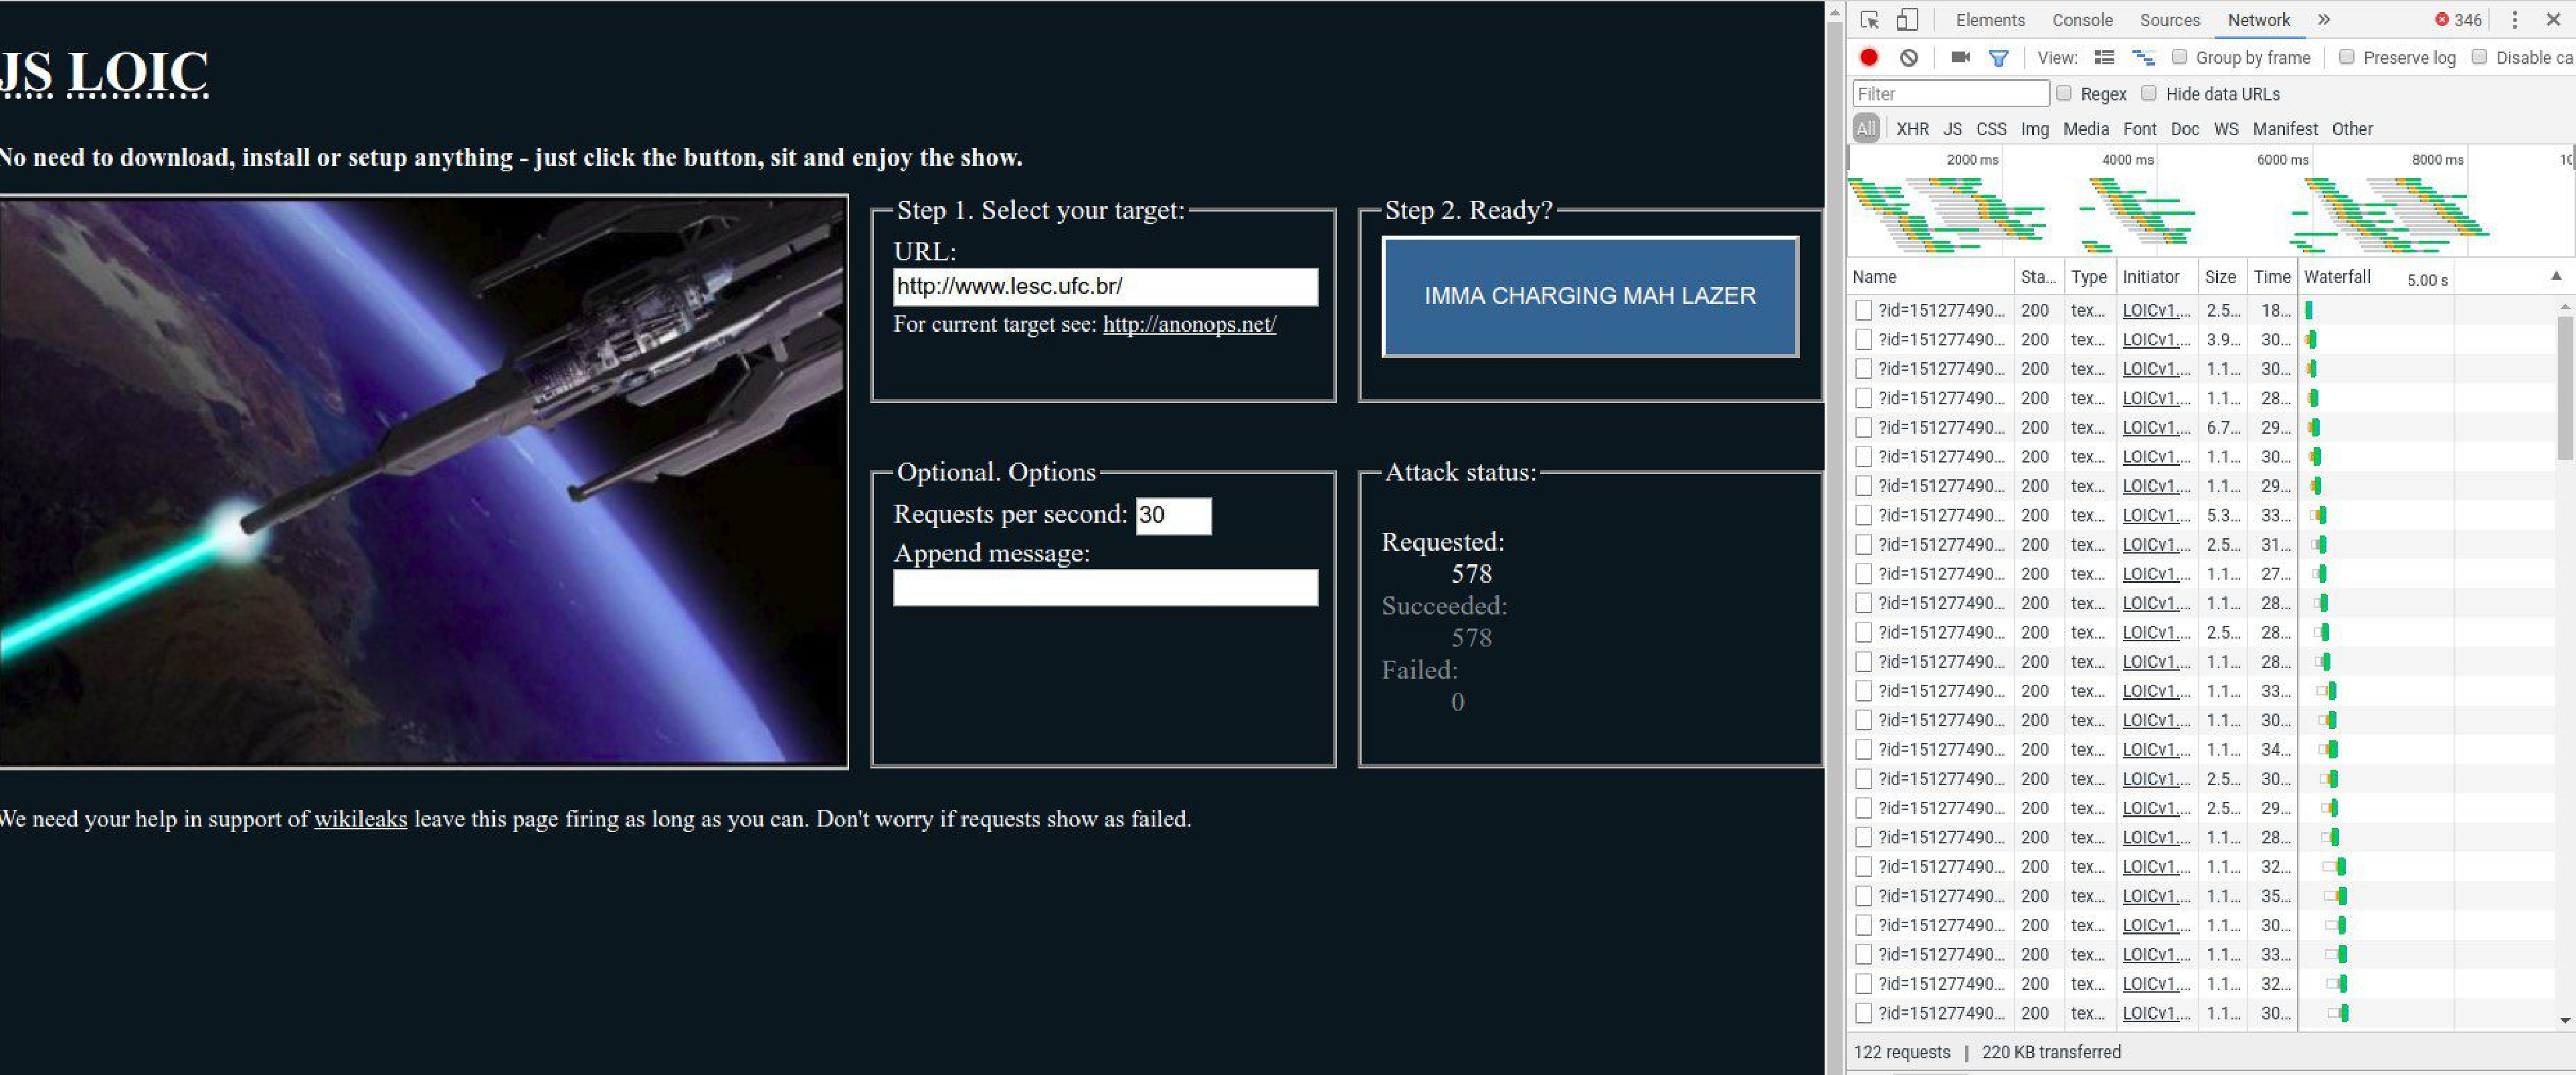
\includegraphics[width=1\textwidth]{figs/loic.pdf}\\
 	{Fonte: http://metacortexsecurity.com/tools/anon/LOIC/LOICv1.html}
 	\label{fig:loic}
 \end{figure} 
 
 A \figref{fig:loic} mostra requisições à direita sendo respondidas com código 200 (OK) pelo servidor alvo, sendo que 30 requisições por segundo são enviadas ao mesmo. Vale ressaltar que o uso de apenas um \textit{host} realizando  esse processo não configura um ataque DDoS, visto que seriam necessárias várias máquinas enviando esse tipo de requisição em uma mesma janela de tempo para causar algum dano ao servidor.
 
 \subsection{UDP \textit{flood}}
 
 Diferentemente do HTTP \textit{flood}, a versão UDP (\textit{User Datagram Protocol}) atua no protocolo da camada de transporte e tem como objetivo congestionar o \textit{link} do alvo. Assim, em um ataque UDP \textit{flood}, uma grande quantidade de pacotes UDP são enviados para as portas do alvo. Para ocultar a identidade do atacante, o mesmo falsifica o endereço IP de origem dos pacotes de ataque. Os ataques de inundação UDP também podem esgotar a largura de banda da rede em torno do sistema da vítima. Por isso, os sistemas em torno da vítima também são impactados devido ao ataque de inundação UDP \cite{xiaoming2010denial}. Segundo \citeonline{ddosatacks}, um ataque UDP \textit{flood} é possível quando um atacante envia um pacote UDP para uma porta aleatória do sistema da vítima. Após isso, quando a vítima recebe esse pacote, ela irá determinar que aplicação está aguardando na porta destino e quando ela percebe que não tem nenhuma aplicação esperando, ela envia um pacote ICMP contendo a mensagem de "destino inalcançável" para o destino cujo IP foi forjado e devido a grande quantidade de pacotes UDP, o sistema alvo irá cair. Uma ferramenta comumente utilizada para esse tipo de ataque é o Trin00 \cite{criscuolo2000distributed}, a qual é responsável por lançar massas de dados UDP para um ou mais endereços IP \cite{dittrich2002projectos}.
 
 
 \subsection{SIDDoS}   
  Outro tipo de ataque DDoS é o SQL \textit{Injection} DDoS, no qual atacantes inserem  requisições SQL (\textit{Structured Query Language}) para o banco de dados da vítima através, por exemplo, de um formulário o qual possui vulnerabilidades (falta de validação das entradas). Então, ilegalmente, permitindo acesso aos recursos ou mesmo aos dados guardados pelo servidor \cite{DataMining}. A maior parte desse tipo de ataque ocorre em telas de \textit{login}, as quais o atacante tem acesso indireto ao banco de dados, através do preenchimento malicioso desses elementos com códigos SQL. Uma ferramenta utilizada para tal fim é o SQLMap, no qual o uso consiste em apenas definir um alvo e o tipo de ataque SQL \textit{Injection}. 

\section{IDS}

Para tratar esse tipo de problema, são utilizados sistemas do tipo IDS (\textit{Intrusion detection System}). Tratam-se de \textit{softwares} responsáveis  por detectar anomalias na rede, como por exemplo acessos não autorizados e tráfegos mal intencionados. Os IDS monitoram o tráfego, buscando anomalias e em caso positivo, alerta aos administradores da rede para que estes tomarem as medidas corretivas, bloqueando as portas, negando serviço a um IP específico que esteja enviando requisições maliciosas ou fechando serviços que são geralmente utilizados para ataques. Segundo \citeonline{ashoor2011importance}, os sistemas IDS possuem 3 categorias: 
\begin{itemize}
	\item Sistemas de detecção baseados em assinatura.
	\item Sistemas de detecção baseados em anomalias.
	\item Sistemas de detecção baseados em especificação.
\end{itemize}

O sistema de detecção baseado em assinaturas representa um ataque conhecido através de um padrão ou assinatura para que os ataques descritos e suas variações sejam identificados. Assim, esse tipo de sistema depende de listas atualizadas com padrões de ataques e assim, será impossível detectar uma ameaça desconhecida ou atualizada. No caso de sistemas baseados em anomalias, é importante que haja uma classificação da rede como normal ou anômala, além de conhecer o comportamento normal da rede. Por fim, um sistema de detecção baseados em especificação é responsável por monitorar os processos e caso detecte qualquer comportamento anormal, emitirá um alerta e deve ser mantido e atualizado sempre que houver alguma alteração.

Assim, os sistemas IDS utilizam alguns conceitos para realizar seus serviços. Pode-se destacar a definição de objeto de tráfego, o qual significa um conjunto de pacotes em uma determinada janela de tempo. A partir de um objeto de tráfego, pode-se calcular métricas de avaliação da rede. Vale ressaltar que para a obtenção de objetos de tráfego, faz-se necessário o uso de \textit{sniffer}, um analisador de rede que captura o tráfego de entrada e saída. Desta forma, os pacotes são capturados e calculam-se os parâmetros do objeto de tráfego.

Alguns IDS podem ser encontrados na literatura. O trabalho em \cite{cabrera2001proactive} utiliza dados da MIB (\textit{Management Information Base}) vinda do roteador para realizar a detecção. Esses dados incluem parâmetros que indicam diferentes estatísticas de pacotes e rotas, focando na identificação de padrões estatísticos de diferentes formas, com o objetivo de realizar a detecção o mais cedo possível. Outro mecanismo chamado CTPS/PF (\textit{Congestion-Triggered Packet Sampling/Packet Filtering}) foi proposto por \cite{huang2001countering}. De acordo com essa abordagem, um subconjunto de pacotes descartados devido ao congestionamento são selecionados para análise estatística. Se uma anomalia é indicada pelos resultados estatísticos, um sinal é enviado ao roteador para filtrar os pacotes maliciosos. No trabalho proposto por \citeonline{multops} é apresentada uma heurística chamada MULTOPS, que postula que se a detecção de endereços IP que participam de um ataque DDoS é possível, então são tomadas medidas para bloquear apenas esses endereços específicos. Cada dispositivo de rede mantém uma árvore de vários níveis que contém estatísticas de taxa de pacotes para prefixos de sub-rede em diferentes níveis de agregação. MULTOPS usa taxas desproporcionais de \textit{hosts} e sub-redes para detectar ataques. Quando armazena as estatísticas com base em endereços de origem, é dito que ele opera em modo orientado a ataques, caso contrário, atua no modo orientado à vítima. Uma estrutura de dados MULTOPS pode assim ser usada para manter o controle de ataques em \textit{hosts}. Quando a taxa de pacote de uma sub-rede atinge um determinado limite, um novo sub-nó é criado para acompanhar as taxas de pacotes mais finas. Esse processo prossegue até que sejam mantidas as taxas de pacotes de endereços IP. Portanto, a partir de uma granularidade grosseira, pode-se detectar mais precisamente a fonte de ataque exata ou os endereços de destino. Já o IDS proposto em \citeonline{HOQUE201748}, no qual esse trabalho é baseado,  propõe-se um \textit{framework} de detecção de ataques DDoS baseado em uma correlação proposta pelos mesmos autores chamada NaHiD, a qual é capaz de verificar a cada segundo, se uma instância de tráfego é normal ou maliciosa. O \textit{framework} possui três componentes: Pré-processamento, Módulo de detecção e gerenciador de segurança. O primeiro é responsável por capturar e filtrar os pacotes em uma janela de um segundo. No módulo de detecção, a correlação será calculada entre um perfil normal pré-estabelecido e o tráfego  em análise. Se 
o  valor da correlação for maior que o limiar também pré-estabelecido, significa que o tráfego analisado tem similaridade alta com um tráfego normal, sendo julgado dessa forma e o \textit{framework} irá atualizar esse perfil normal. Caso contrário, o tráfego será atribuído como um ataque. O gerenciador de segurança  salva as estatísticas de tráfego de rede, bem como os valores calculados em \textit{logs}. A medida de correlação NaHiD leva em consideração três parâmetros: Entropia e Variação de IPs origem e taxa de pacotes. A entropia é calculada baseada na fórmula de Shannon, a qual mede o grau de desorganização de um conjunto. Já na variação de IPs origem, tem-se que cada variação de um IP origem em um conjunto de pacotes deve ser incrementada. Por tratar-se de detecção em tempo real, os autores propuseram o cálculo da correlação NaHiD em \textit{hardware} (FPGA), pois o tempo de detecção cairia drasticamente com essa modificação. Assim, tal correlação apresentou baixo tempo de processamento entre a detecção em \textit{hardware} e \textit{software}, sendo da ordem de 1 microssegundo para identificar um tráfego.  
 


%Falar sobre ataques, definir objeto de tráfego, sniffer IDS vulnerabilidades trabalhos relacionaados entropia de shaannon... EXEMPLOS DE AATQUES ddos IIDS Q TEM NO PAPER ORIGINAL FALAR SOBRE
   

